In the posterior predictive model checking of this study (Section~\ref{subsec:wo Layers of Model Checking}), we found that the \textbf{maximum survey duration $A$}, controlling the censoring mechanism in Algorithm 1 through the reparameterization $A$, has a substantial influence on simulation outcomes and the credibility of posterior predictive results. In simulation, $A$ defines the observation window, thereby determining both the censoring rate and the distribution of event times. Although $A$ is not estimated by the baseline model, it is a key external setting when generating fake data. Different choices of $A$ alter the censoring structure and can change the conclusions drawn from posterior predictive checks, making $A$ tightly coupled with model checking~\cite{stats5010006}.

Does the observed data carry information about $A$? Yes. In any survival dataset, the “shadow” of the survey window is reflected in the censoring proportion and the shape of the observed durations~\cite{barrajón2020effectrightcensoringbias, stats5010006, bartovs2022informed}. If $A$ is small, many subjects are censored before the event occurs, leading to a high right-censoring rate and “compressed” event times. Conversely, a large $A$ yields more observed events, lower censoring, and more dispersed event times.

\begin{example}
Figure~\ref{fig:离职数据分开的直方图} separates event and censored durations in the employee turnover data. The roughly balanced counts suggest the survey captured about half of the departures. Since the maximum observed duration exceeds 179 months, the survey-length parameter $A$ should be at least above this threshold. While this alone does not determine $A$, it provides a lower bound and motivates exploring its impact on model fit. Such heuristic information, although limited, points to the need for a Bayesian formulation~\cite{bartovs2022informed} in which $A$ can be explicitly incorporated into the likelihood and estimated jointly with event-time parameters. 
\begin{figure}[H]
    \centering
    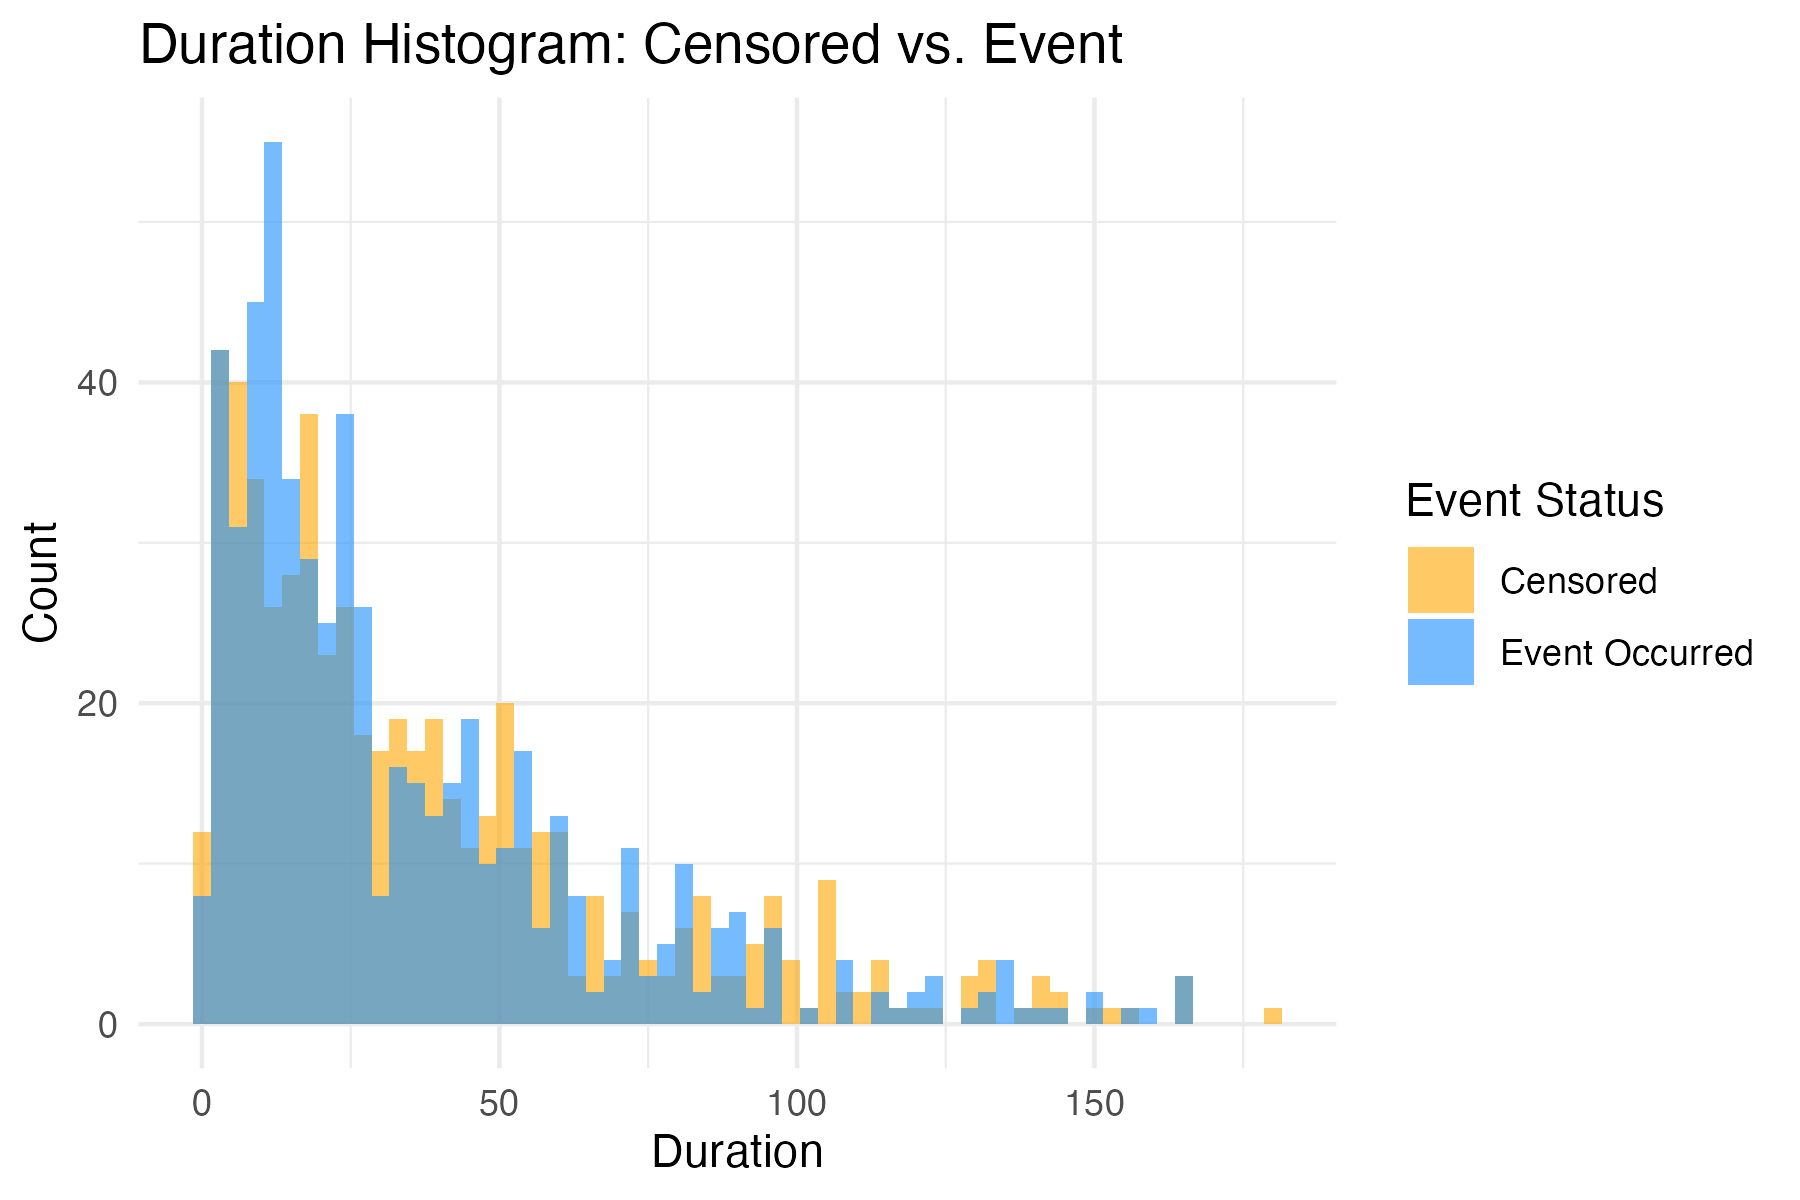
\includegraphics[height=5.5cm, width=0.6\textwidth]{images/separate_hist.png}
    \caption{{\small Histograms of censored and event durations in the employee turnover data}}
    \label{fig:离职数据分开的直方图}
\end{figure}
To illustrate the effect of unrealistic observation windows, we simulate under three settings, $A = 30$, $A = 200$, and $A = 1000$, and plot the corresponding histograms of event times ($\delta = 1$) and censored times ($\delta = 0$). These examples serve as a motivating illustration of how the choice of $A$ shapes the distribution of observed durations.
\begin{itemize}
    \item $A = 30$ (Figure~\ref{fig:fake-hist_a30}): produces durations tightly compressed within a short window, 
    with both events and censorings occurring unusually early.
    \item $A = 200$ (Figure~\ref{fig:fake-hist_a200}): yields a distribution that roughly matches the observed data range 
    (Figure~\ref{fig:离职数据分开的直方图}), providing a plausible intermediate benchmark.
    \item $A = 1000$ (Figure~\ref{fig:fake-hist_a1000}): generates unrealistically dispersed durations extending over several decades, well beyond typical employment spans.
\end{itemize}

\begin{figure}[H]
\centering
\begin{subfigure}[t]{0.45\textwidth}
  \centering
  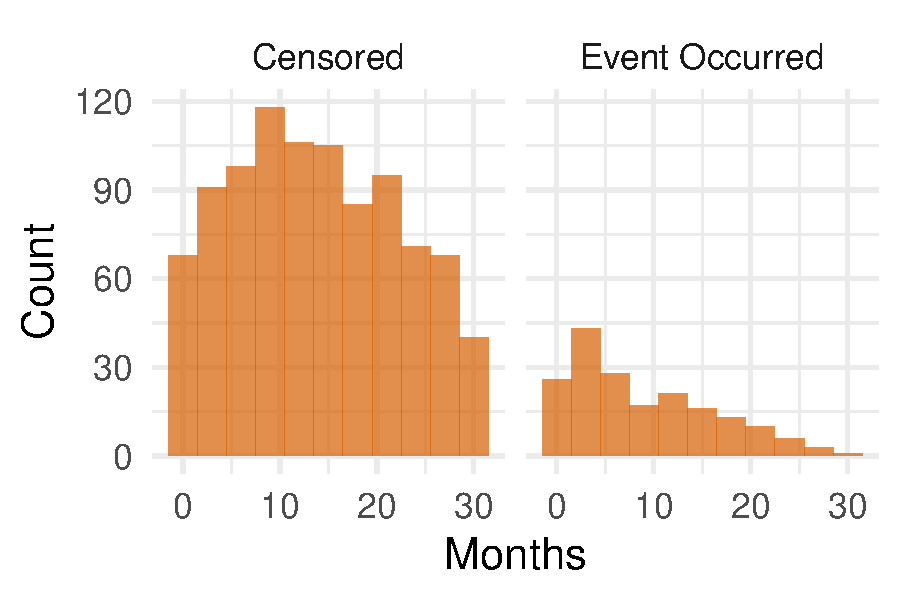
\includegraphics[height=5.5cm,width=\linewidth]{images/fake_duration_hist_a30.pdf}   % 图3路径
  \caption{{\small $A=30$ months — compressed durations}}
  \label{fig:fake-hist_a30}
\end{subfigure}
\begin{subfigure}[t]{0.45\textwidth}
  \centering
  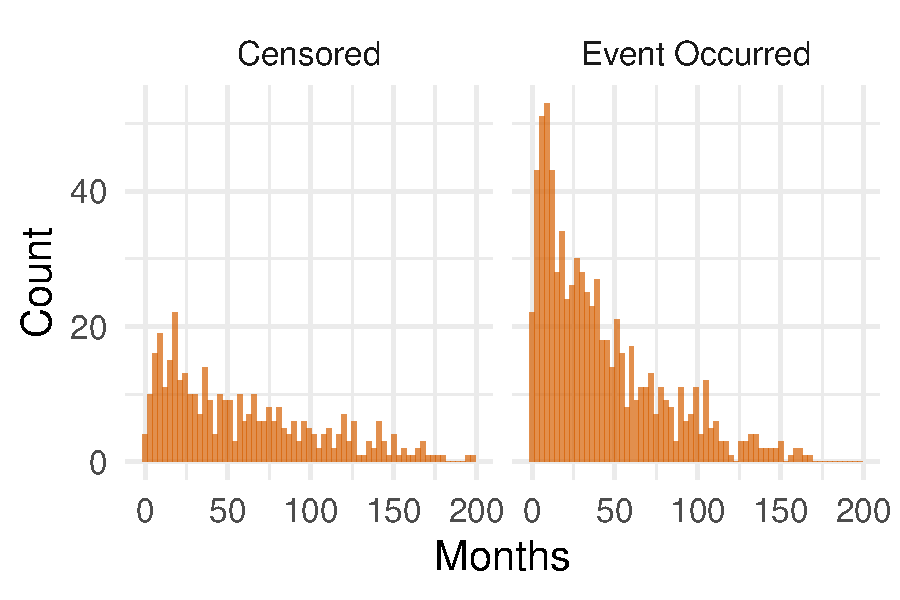
\includegraphics[height=5.5cm,width=\linewidth]{images/fake_duration_hist_a200.pdf}   % 图3路径
  \caption{{\small $A=200$ months — plausible spread}}
  \label{fig:fake-hist_a200}
\end{subfigure}
\begin{subfigure}[t]{0.5\textwidth}
  \centering
  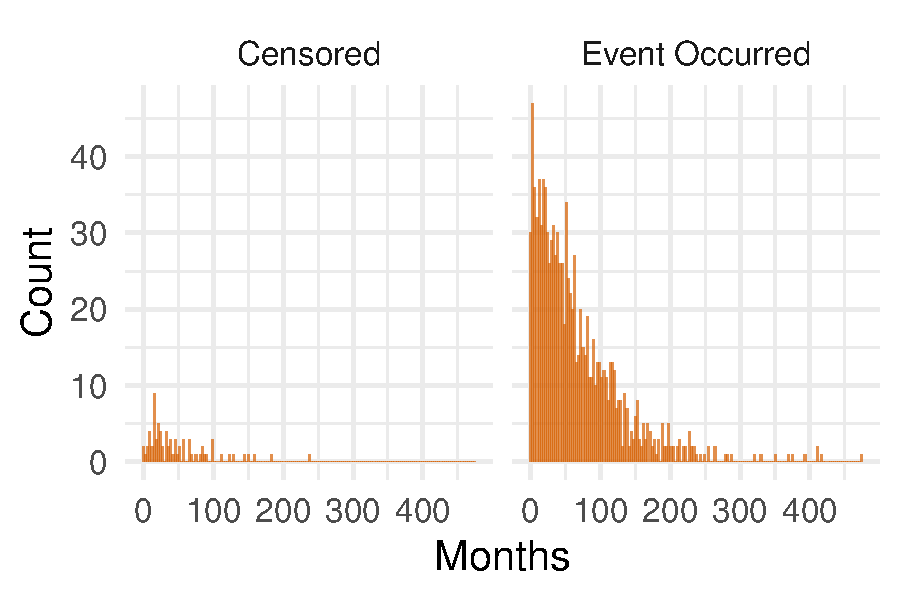
\includegraphics[height=5.5cm,width=\linewidth]{images/fake_duration_hist_a1000.pdf}   % 图3路径
  \caption{{\small $A=1000$ months — implausibly long tails}}
  \label{fig:fake-hist_a1000}
\end{subfigure}
\caption{{\small \textbf{Motivating example:} Simulated histograms under $A=30,200,1000$ months. Full ECDF-based evaluation in Section~\ref{ecdf的分析}.}}
\label{fig:ppc-A30}
\end{figure}
These examples underscore that posterior predictive fit must be interpreted in light of the plausibility of data-generating assumptions. Determining a realistic range for $A$ is essential for credible model checking, and this motivates the next step—explicitly incorporating $A$ into the likelihood and estimating it jointly with event-time parameters.
\end{example}